\documentclass{icga}
\newif\iflong\longfalse  %change to longtrue for longer version
% additional long version material like this:
% \iflong
% ... long version material ...
% \fi

\usepackage{url}
\usepackage{graphicx}
\def\Eo{\mbox{\sc Ezo}}
\def\Hz{\mbox{\sc Hexamaze}}
\def\Mx{\mbox{\sc MoHex}}
\def\Mt{\mbox{\sc MoHexNet}}
\def\Nx{\mbox{\sc NeuroHex}}
\def\Sol{\mbox{\sc Solver}}
\def\Fuego{\mbox{\sc Fuego}}
\def\TV{\mbox{\sc TV}} %Tony van der Valk

\title{\sc MOHEX WINS HEX 11x11 AND 13x13 TOURNAMENTS}
\runningtitle{ICGA}
\author{Ryan Hayward\thanks{Department 
of Computing Science, University of Alberta, Canada. Email:hayward@ualberta.ca},
Noah Weninger \thanks{CS, UAlberta, Email:nweninge@ualberta.ca},
Kenny Young\thanks{CS, UAlberta. Email:kjyoung@ualberta.ca},
Kei Takada \thanks{takada@complex.ist.hokudai.ac.jp} and
Tianli Zhang \thanks{zhtl1995@gmail.com}
}
\affiliation{Edmonton, Canada}
\issue{???}

\setcounter{page}{999}
\begin{document}
\maketitle

\iflong
In the longer version of the report, we include all games.
\fi

\vspace*{-2.25in}
%{\it ICGA Journal Vol.\ XX No.\ YY Sept 999 pp ??-??
%\hfill Computer Games Olympiad, 2016 Leiden.}
{\it to appear, ICGA Journal}
\vspace*{2.0in}

\begin{figure}[hbt]
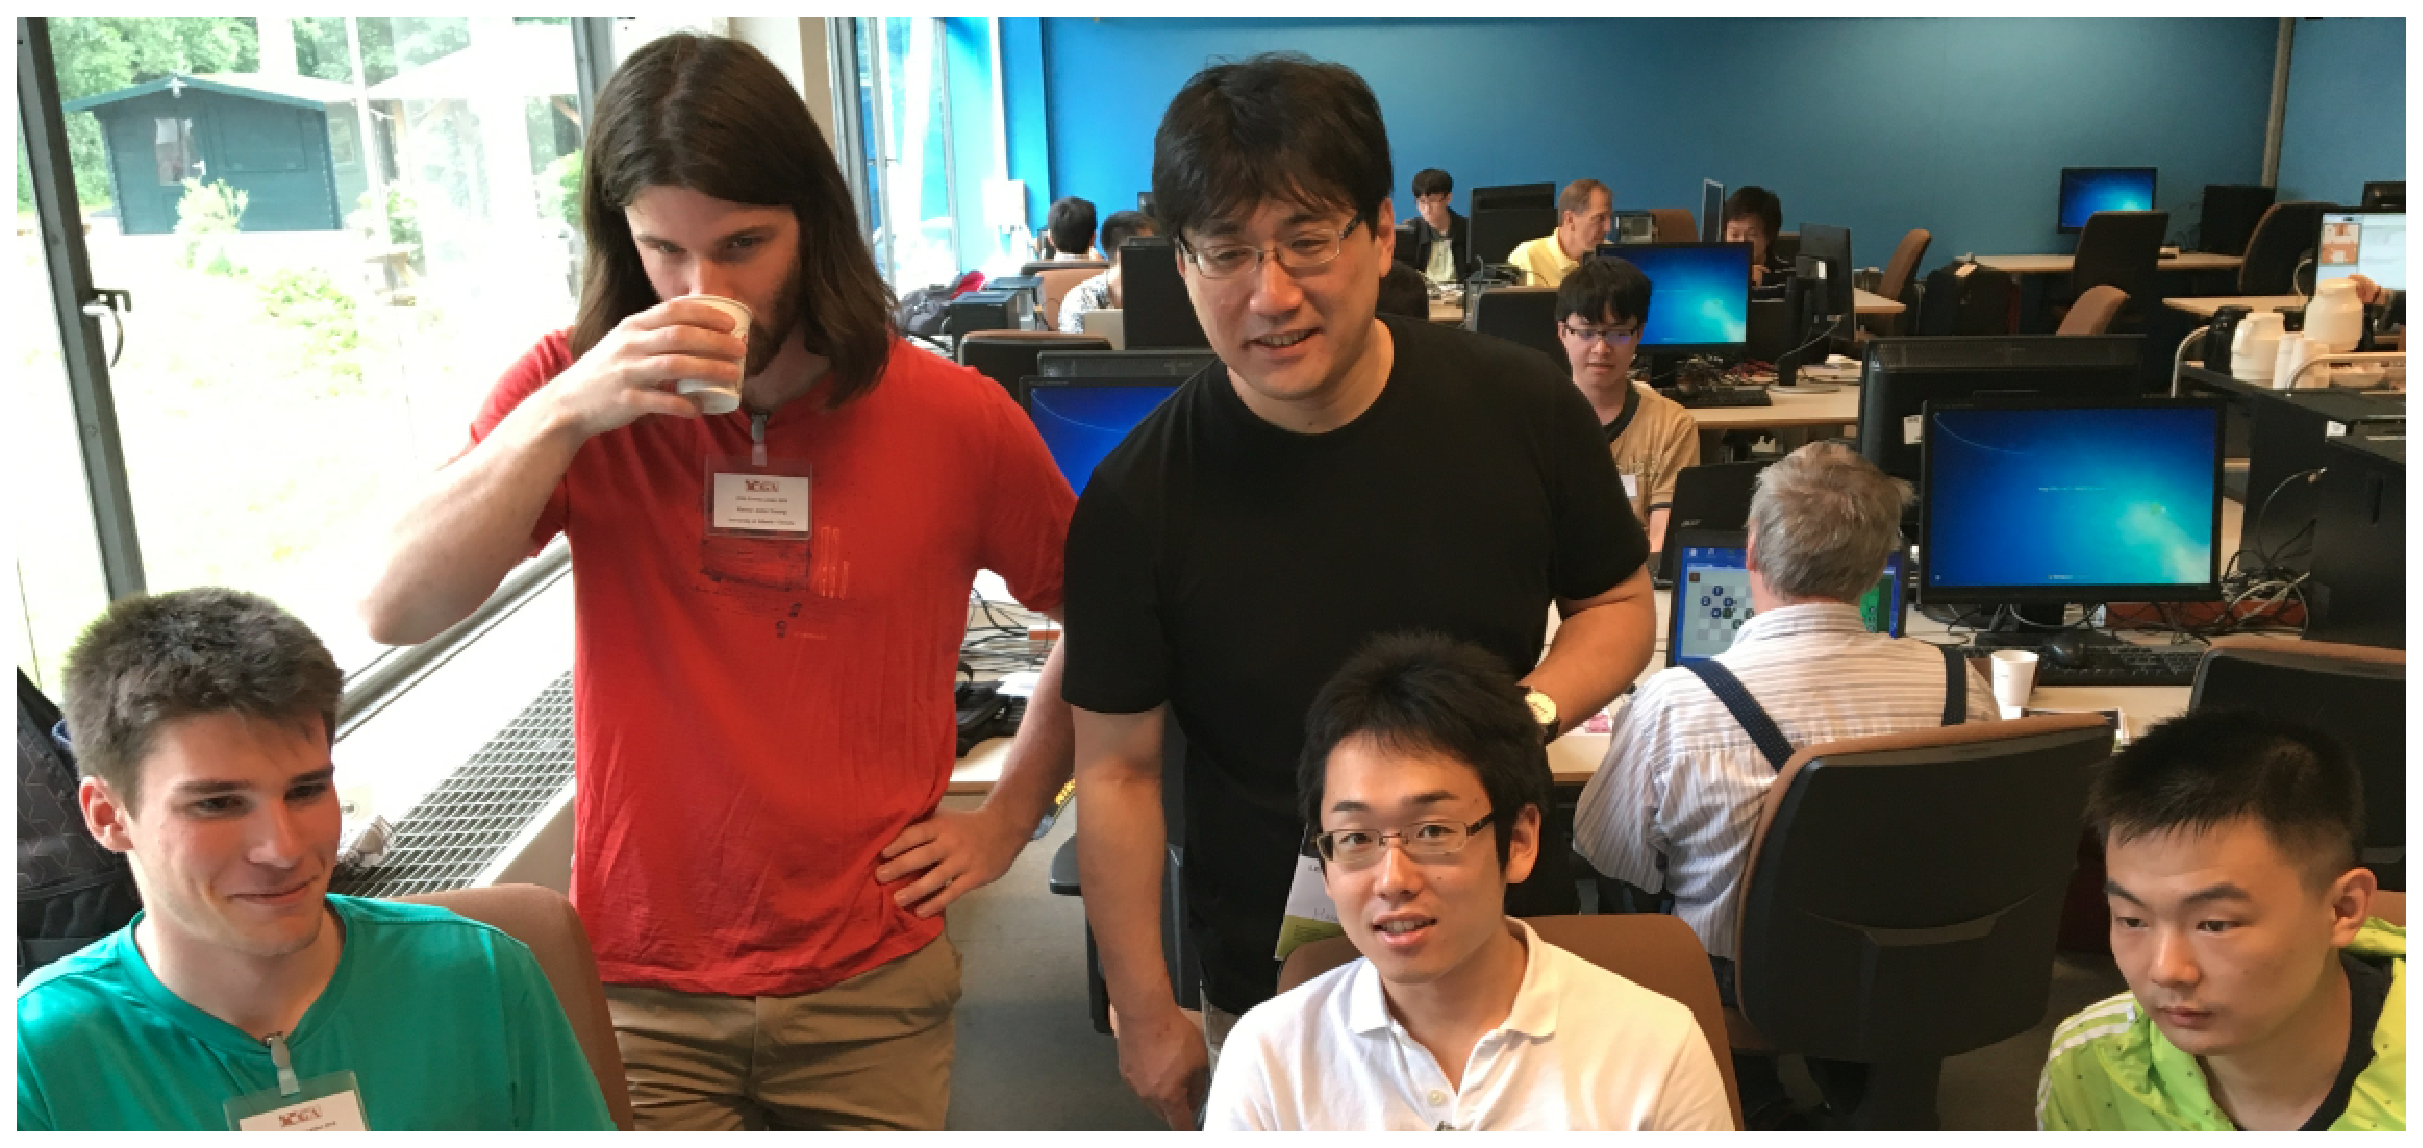
\includegraphics[width=225pt]{photos/pick.eps}\
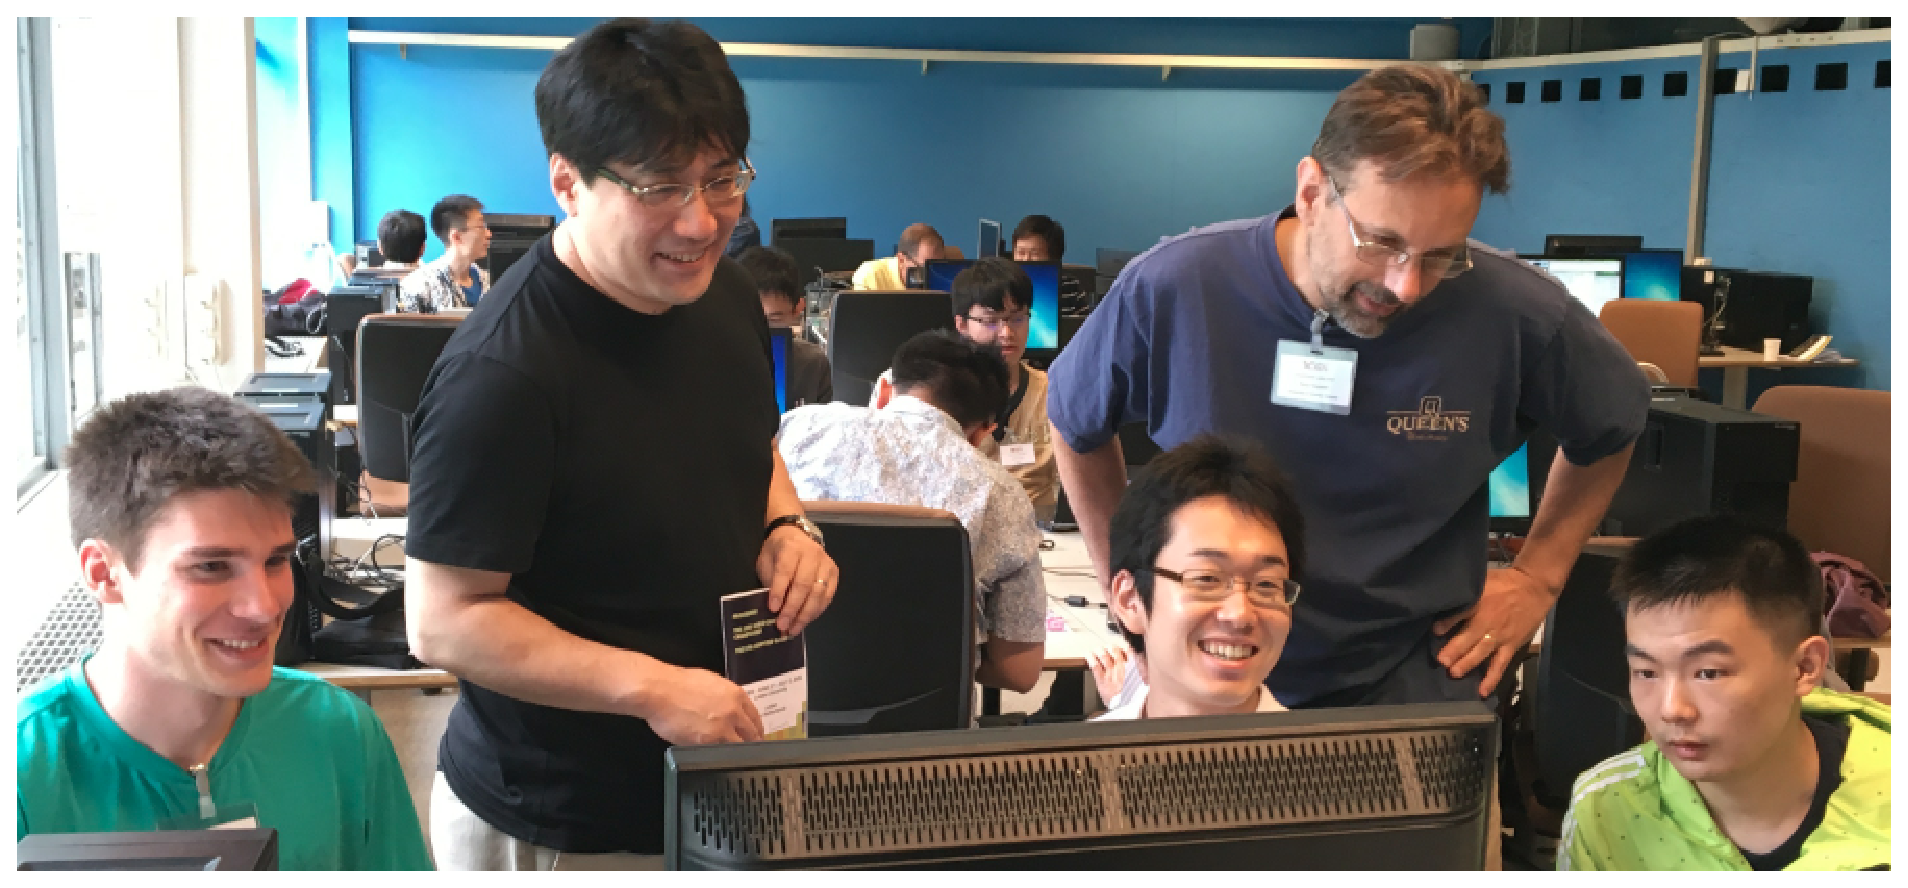
\includegraphics[width=225pt]{photos/picr.eps}
\caption{Participants and observers at the Hex competitions.}
\end{figure}

\section{The Tournaments}
There were two Hex tournaments at the 2016 Olympiad:
board size 11$\times$11 and board size 13$\times$13.
Three programs competed in each tournament:
\Eo{} by Kei Takada, supervised by Masahito Yamamoto, from Japan;
\Hz{} by Tianli Zhang from China; and
\Mx{} 2.0 \citebay{HAHMP13}, 
by Broderick Arneson, Ryan Hayward, Philip Henderson, Aja Huang, 
Jakub Pawlewicz, Noah Weninger, and Kenny Young from Canada.

\Mx{}, the winner of the previous six Olympiad Hex competitions
\citebay{HAHP13},
is an MCTS program that uses the Benzene Hex framework
built on the code base of \Fuego\ \citebay{fuego}.
%the Go program developed by Martin M\"{u}ller, Markus Enzenberger
%and others at the University of Alberta.
%Benzene allows virtual connection and
%inferior cell computations.
\Mx{} performs knowledge computation in UCT tree nodes visited at least 256 times.
\Mx{} ran on Firecreek, a 24 core shared-memory machine, 
with 4 cores reserved for the 
DFPNS solver \citebay{PawlH13}, which
produces perfect play if it solves the
position within the time allotted.
\Mx{} uses a book ---
built by Broderick Arneson with Thomas Lincke's method 
\citebay{DBLP:conf/cg/Lincke00}. 
Noah Weninger expanded the book and added a feature
allowing the use of rotational symmetry for openings
whose rotation is in the book.
For each board size, the book covers at least eight openings.

\Eo{} is a stronger version of the program that competed in the 2015 Olympiad.
\Eo{}, now based on the Benzene framework, 
uses iterative deepening depth-first search 
with an evaluation function using a linear combination of
two network connectivity measures \citebay{TakadaHIY15}.
\Eo{} ran on two threads of an i7 4790 laptop,
with one thread for search and one thread for
Benzene's Depth-First Proof Number Search endgame solver.

\Hz{} is a new MCTS program written by Tianli Zhang from 
Beijing Institute of Technology.

Each tournament was a three-player double round robin, so 12 games
in total with 8 games per player.

{\large\bf 11$\times$11 Tournament.}\footnote{Source files for this report, including .sgf files, at \url{https://github.com/ryanbhayward/icga-olympiad-hex}.}
The tournment took place on June 26 and 27.
The final two scheduled games were not played,
as by then the outcome had been decided.
After the tournament, \Mx\ and \Eo\ played two 
exhibition same-resource games,
with one thread for the search and one
thread for the solver. They each won one game.
In the tournament, the operator usually resigned
once the Benzene solver detected a win or loss.

\hfill\begin{tabular}{|c|c|c|c|c|c|}
\hline 11x11 results &\Mx{} &\Eo{}  & \Hz{}  & total & result \\ 
\hline \Mx{}         &      &  4-0  &  3-0   & 7-0  &  gold \\
\hline \Eo{}         &  0-4 &       &  3-0   & 3-4  &  silver \\
\hline \Hz{}         &  0-3 &  0-3  &        & 0-6  &  bronze \\
\hline
\end{tabular}\hfill~

\iflong
This is the longer version, so we include all games.
\fi


%{\bf Game 1.}
%{\sc E-M 0-1.}
%1.B[a9] 2.W[b10] 3.B[f7] \ldots ~ ~ 
%
%{\bf Game 2.}
%{\sc M-H 1-0.}
%1.B[a2] 2.W[b9] 3.B[e7] \ldots ~ ~ 
%
%{\bf Game 3.}
%{\sc H-E 0-1.}
%1.B[a2] 2.W[swap] 3.B[g5] \ldots ~ ~ 
%
%{\bf Game 4.}
%{\sc M-E 1-0.}
%1.B[a6] 2.W[c9] 3.B[g7] \ldots ~ ~ 
%
%{\bf Game 5.}
%{\sc H-M 0-1.}
%1.B[a2] 2.W[g5] 3.B[f5] \ldots ~ ~ 
%
%{\bf Game 6.}
%{\sc E-H 1-0.}
%1.B[a2] 2.W[b9] 3.B[e7] \ldots ~ ~ 
%
%{\bf Game 7.}
%{\sc E-M 0-1.}
%1.B[k5] 2.W[e7] 3.B[g6] \ldots ~ ~ 
%
%{\bf Game 8.}
%{\sc M-H 1-0.}
%1.B[a7] 2.W[swap] 3.B[g5] \ldots ~ ~ 
%
%{\bf Game 9.}
%{\sc H-E 0-1.}
%1.B[a2] 2.W[swap] 3.B[j3] \ldots ~ ~ 
%
%{\bf Game 10.}
%{\sc M-E 1-0.}
%1.B[a6] 2.W[c9] 3.B[g7] \ldots ~ ~ 
%
%\begin{figure}[hbp]
%\includegraphics[scale=1.3]{games/pix/01-em-0-1.eps}\hspace*{-1cm}\
%\includegraphics[scale=1.3]{games/pix/01-em-completion.eps}\
%\caption{Game 1: \Eo-\Mx\ 0-1. Black resigned after move 34 (on left), when it saw the loss.}
%\end{figure}
%
%\begin{figure}[hbp]
%\includegraphics[scale=1.3]{games/pix/10-me-1-0.eps}\hspace*{-1cm}\
%\includegraphics[scale=1.3]{games/pix/10-me-completion.eps}
%\caption{Game 10: \Mx-\Eo\ 1-0. Black resigned after move 38 (on left), when it saw the loss.}
%\end{figure}

\begin{figure}[hbp]
\hspace*{-2.5cm}\
%\includegraphics[scale=1.3]{games/pix/01-em-0-1.eps}\hspace*{-2cm}\
\includegraphics[scale=1.2]{games/pix/01-em-completion.eps}\hspace*{-2cm}\
\includegraphics[scale=1.2]{games/pix/02-mh-1-0.eps}\hspace*{-2cm}\
\includegraphics[scale=1.2]{games/pix/03-he-0-1.eps}
\caption{Game 1: \Eo-\Mx\ 0-1. Game 2: \Mx-\Hz\ 1-0. Game 3: \Hz-\Eo\ 0-1.} 
\end{figure}

\begin{figure}[hbp]
\hspace*{-2.5cm}\
\includegraphics[scale=1.2]{games/pix/04-me-1-0.eps}\hspace*{-2cm}\
\includegraphics[scale=1.2]{games/pix/05-hm-0-1.eps}\hspace*{-2cm}\
\includegraphics[scale=1.2]{games/pix/06-eh-1-0.eps}
\caption{Game 4: \Mx-\Eo\ 1-0. Game 5: \Hz-\Mx\ 0-1. Game 6: \Eo-\Hz\ 1-0.}
\end{figure}

\begin{figure}[hbp]
\hspace*{-2cm}\
\includegraphics[scale=1.2]{games/pix/07-em-0-1.eps}\hspace*{-2cm}\
\includegraphics[scale=1.2]{games/pix/08-mh-1-0.eps}\hspace*{-2cm}\
\includegraphics[scale=1.2]{games/pix/09-he-0-1.eps}
\caption{Game 7: \Eo-\Mx\ 0-1. Game 8: \Mx-\Hz\ 1-0. Game 9: \Hz-\Eo\ 0-1.}
\end{figure}

\begin{figure}[hbp]
\hspace*{-2cm}\
%\includegraphics[scale=1.3]{games/pix/10-me-1-0.eps}\hspace*{-2cm}\
\includegraphics[scale=1.2]{games/pix/10-me-completion.eps}\hspace*{-2cm}\
\includegraphics[scale=1.2]{games/pix/em-friendly-0-1.eps}\hspace*{-2cm}\
\includegraphics[scale=1.2]{games/pix/me-friendly-0-1.eps}
\caption{Game 10: \Mx-\Eo\ 1-0. Exhibition 1-thread games: \Eo-\Mx\ 0-1, \Mx-\Eo\ 0-1.}
\end{figure}

~

{\large\bf 13$\times$13 Tournament.}
The tournament took place on June 30 and July 1.
As with 11$\times$11, there was clear separation
between each pair of players.
In games 10 and 12 \Mx\ played first in the centre,
allowing the opponent to swap and take what is presumably
the strongest possible opening move.

\hfill\begin{tabular}{|c|c|c|c|c|c|}
\hline 13x13 results &\Mx{} &\Eo{}  &\Hz{} & total & result \\ 
\hline \Mt{}         &      &  4-0  & 4-0  & 8-0   & gold \\
\hline \Eo{}         &  0-4 &       & 4-0  & 4-4   & silver \\
\hline \Hz{}         &  0-4 &  0-4  &      & 0-8   & bronze \\
\hline
\end{tabular}\hfill~

%{\bf Game 1.}
%{\sc E-M 0-1.}
%1.B[?] 2.W[?] 3.B[?] \ldots ~ ~ 
%
%{\bf Game 2.}
%{\sc M-H 1-0.}
%1.B[?] 2.W[?] 3.B[?] \ldots ~ ~ 
%
%{\bf Game 3.}
%{\sc H-E 0-1.}
%1.B[?] 2.W[?] 3.B[?] \ldots ~ ~ 
%
%{\bf Game 4.}
%{\sc M-E 1-0.}
%1.B[?] 2.W[?] 3.B[?] \ldots ~ ~ 
%
%{\bf Game 5.}
%{\sc H-M 0-1.}
%1.B[?] 2.W[?] 3.B[?] \ldots ~ ~ 
%
%{\bf Game 6.}
%{\sc E-H 1-0.}
%1.B[?] 2.W[?] 3.B[?] \ldots ~ ~ 
%
%{\bf Game 7.}
%{\sc E-M 0-1.}
%1.B[?] 2.W[?] 3.B[?] \ldots ~ ~ 
%
%{\bf Game 8.}
%{\sc M-H 1-0.}
%1.B[?] 2.W[?] 3.B[?] \ldots ~ ~ 
%
%{\bf Game 9.}
%{\sc H-E 0-1.}
%1.B[?] 2.W[?] 3.B[?] \ldots ~ ~ 
%
%{\bf Game 10.}
%{\sc M-E 1-0.}
%1.B[?] 2.W[?] 3.B[?] \ldots ~ ~ 
%
%{\bf Game 11.}
%{\sc H-M 0-1.}
%1.B[?] 2.W[?] 3.B[?] \ldots ~ ~ 
%
%{\bf Game 12.}
%{\sc E-H 1-0.}
%1.B[?] 2.W[?] 3.B[?] \ldots ~ ~ 

\begin{figure}[hbp]
\hspace*{-2cm}\
\includegraphics[scale=1.1]{games/pix/13-01-em-0-1.eps}\hspace*{-2cm}\
\includegraphics[scale=1.1]{games/pix/13-02-mh-1-0.eps}\hspace*{-2cm}\
\includegraphics[scale=1.1]{games/pix/13-03-he-0-1.eps}
\caption{Game 1: \Eo-\Mx\ 0-1. Game 2: \Mx-\Hz\ 1-0. Game 3: \Hz-\Eo\ 0-1.}
\end{figure}

\begin{figure}[hbp]
\hspace*{-2cm}\
\includegraphics[scale=1.1]{games/pix/13-04-me-1-0.eps}\hspace*{-2cm}\
\includegraphics[scale=1.1]{games/pix/13-05-hm-0-1.eps}\hspace*{-2cm}\
\includegraphics[scale=1.1]{games/pix/13-06-eh-1-0.eps}
\caption{Game 4: \Mx-\Eo\ 1-0. Game 5: \Hz-\Mx\ 0-1. Game 6: \Eo-\Hz\ 1-0.}
\end{figure}

\begin{figure}[hbp]
\hspace*{-2cm}\
\includegraphics[scale=1.1]{games/pix/13-07-em-0-1.eps}\hspace*{-2cm}\
\includegraphics[scale=1.1]{games/pix/13-08-mh-1-0.eps}\hspace*{-2cm}\
\includegraphics[scale=1.1]{games/pix/13-09-he-0-1.eps}
\caption{Game 7: \Eo-\Mx\ 0-1. Game 8: \Mx-\Hz\ 1-0. Game 9: \Hz-\Eo\ 0-1.}
\end{figure}

\begin{figure}[hbp]
\hspace*{-2cm}\
\includegraphics[scale=1.1]{games/pix/13-10-me-1-0.eps}\hspace*{-2cm}\
\includegraphics[scale=1.1]{games/pix/13-11-hm-0-1.eps}\hspace*{-2cm}\
\includegraphics[scale=1.1]{games/pix/13-12-eh-1-0.eps}
\caption{Game 10: \Mx-\Eo\ 1-0. Game 11: \Hz-\Mx\ 0-1. Game 12: \Eo-\Hz\ 1-0.}
\end{figure}

\section{Conclusions}
In pre-tournament tests,
\Eo\ won 65\% of its games against 1-thread \Mx,
but here the 20-thread search of \Mx\ was too strong.
\Hz\ played well when allowed the centre against \Mx,
forcing a long game.

The next step is to add neural nets.
For this tournament,
the \Mx\ team prepared \Mt{}, a program that combines the
MCTS tree and a depth-1 tree found by \Nx{}, 
a Deep Convolution Neural Net \citebay{YoungVH16}.
On typical swap-game openings,
\Mt\ wins 55\% of its games against \Mx,
a small first step towards an AlphaGo-style player.

{\bf Acknowledgements.}
We thank the NSERC Discovery Grant Program for research funding and
Martin M\"{u}ller for the loan of his machine Firecreek.
\bibliography{rpt}
\end{document}
